\documentclass{article}
\usepackage[T1]{fontenc}
\usepackage{lmodern}
\usepackage{graphicx}
\usepackage{amsmath,amssymb}
\usepackage[a4paper,margin=2cm]{geometry}
\usepackage[absolute,overlay]{textpos}
\setlength{\TPHorizModule}{1mm}
\setlength{\TPVertModule}{1mm}
\usepackage[indonesian]{babel}
\usepackage{hyperref}
\setlength{\emergencystretch}{2em}
% unit: Halaman 44

\begin{document}

% === Halaman 44 (llm) ===

\section*{Key-Scheduling Algorithm (KSA)}

\begin{enumerate}
    \item Inisialisasi larik $\text{S}: \text{S}_0 = 0, \text{S}_1 = 1, ..., \text{S}_{255} = 255$

    \vspace{10mm}

    \begin{verbatim}
    for i <- 0 to 255 do
        S[i] <- i
    end
    \end{verbatim}
\end{enumerate}

% deskripsi: Representasi visual array S yang diinisialisasi dengan nilai urut dari 0 sampai 255
% bbox normalisasi: [0.1200, 0.7000, 0.7680, 0.8050]
\begin{textblock*}{136.08mm}(25.20mm,207.90mm)
\noindent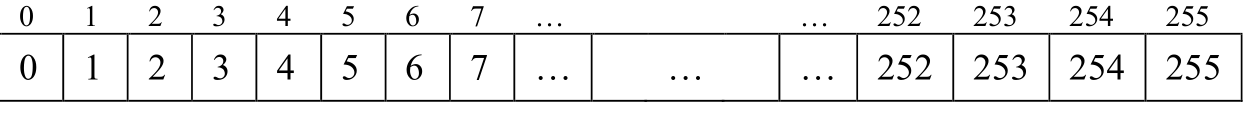
\includegraphics[width=136.08mm,height=31.19mm]{../../images/llm/page_044_img_01.png}%
\end{textblock*}

\end{document}
